\section{Outils pour la virtualisation légère}
\label{section:tools}

Afin d'intercepter les actions d'une application il faut d'abord choisir à quel
niveau se placer.  En effet, une application peut communiquer avec le noyau via
différentes abstractions, comme le montre la Figure \ref{AS_Communication}. Elle
peut soit utiliser les fonctions d'interaction directe avec le noyau que sont
les appels systèmes, soit utiliser les différentes abstractions fournies par le
système d'exploitation: les bibliothèques (fonctions de la \texttt{libc},
bibliothèques de haut niveau telle que \texttt{gtk} par exemples) ou les
fonctions POSIX dans le cas d'un système UNIX.

\begin{figure}[H]
 \centering
 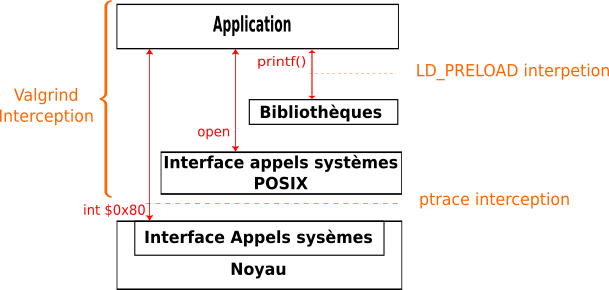
\includegraphics[scale=0.75]{Pictures/png/Communication_application_noyau_v3.png}
 \caption{Communications possibles entre le noyau et une application}
 \label{AS_Communication}
\end{figure}

Nous allons donc voir comment on peut intercepter et modifier des actions au
niveau de l'application (fichier source puis binaire), des appels système et
des appels de fonctions. Par la suite nous appellerons médiation l'ensemble des
modifications effectuées par l'émulateur sur les actions interceptées.

